\documentclass[12pt,oneside,english]{book} 
\usepackage[T1]{fontenc}

% new Lib
\usepackage{algorithm} 
\usepackage{algorithmic}  

\usepackage{fancybox}
\usepackage[algo2e]{algorithm2e} 
\usepackage[Sonny]{fncychap}
\usepackage{float}
\usepackage{wrapfig}  
\usepackage{babel}
%%\usepackage[colorlinks,hyperindex,bookmarks,linkcolor=black,citecolor=blue,urlcolor=black{hyperref}
\usepackage[latin9]{inputenc}
\usepackage{amsmath} 
\usepackage{lscape}
\usepackage{pdflscape}
\usepackage{wasysym}
% end new lib
 

\usepackage{listings}
\usepackage[a4paper]{geometry}
\geometry{verbose,tmargin=2cm,bmargin=2cm,lmargin=3cm,rmargin=2cm,headheight=18pt}
\usepackage{fancyhdr}
\pagestyle{fancy}
\setcounter{secnumdepth}{3}
\setcounter{tocdepth}{3}   

\makeatletter
\addto\extrasfrench{%
   \providecommand{\og}{\leavevmode\flqq~}%
   \providecommand{\fg}{\ifdim\lastskip>\z@\unskip\fi~\frqq}%
}

\makeatother
\usepackage{booktabs}
\usepackage{array}
\usepackage{pifont}
\usepackage{float}
\usepackage{textcomp}
\usepackage{amstext}
\usepackage{amssymb}
\usepackage{graphicx}
\usepackage{setspace}
\onehalfspacing
\usepackage[unicode=true,bookmarks=true,bookmarksnumbered=true,bookmarksopen=true,bookmarksopenlevel=1,
 breaklinks=true,pdfborder={0 0 0},backref=false,colorlinks=false]
 {hyperref}
\hypersetup{pdftitle={Application of the P-graph Methodology for Organization-Based Multi Agent System Designs,A graph Transformation  approach},
 pdfauthor={Nouar Kherkhachi Houssam},
 pdfkeywords={Framework OMACS PNS AToM3 Transformation GraphGrammer Rules Optimisation BranchAndBound}}

\makeatletter

%%%%%%%%%%%%%%%%%%%%%%%%%%%%%% LyX specific LaTeX commands.
%% Because html converters don't know tabularnewline
\providecommand{\tabularnewline}{\\}

%%%%%%%%%%%%%%%%%%%%%%%%%%%%%% User specified LaTeX commands.
\usepackage{cite}
\usepackage{verbatim}


\usepackage{color}
\definecolor{codegreen}{rgb}{0,0.6,0}
\definecolor{codegray}{rgb}{0.1,0.1,0.1}
\definecolor{codepurple}{rgb}{0.58,0,0.82}
\definecolor{backcolour}{rgb}{0.95,0.95,0.92}
 
\lstdefinestyle{mystyle}{
    backgroundcolor=\color{backcolour},   
    commentstyle=\color{codegreen},
    keywordstyle=\color{magenta},
    numberstyle=\color{codegray},%\tiny
    stringstyle=\color{codepurple},
    basicstyle=\footnotesize{},
    breakatwhitespace=false,         
    breaklines=true,                 
    captionpos=b,                    
    keepspaces=true,                 
    numbers=left,                    
    numbersep=5pt,                  
    showspaces=false,                
    showstringspaces=false,
    showtabs=false,                  
    tabsize=2
} 
\lstset{style=mystyle}



\@ifundefined{showcaptionsetup}{}{%
 \PassOptionsToPackage{caption=false}{subfig}}
\usepackage{subfig}
\AtBeginDocument{
  \def\labelitemi{\ding{113}}
  \def\labelitemii{\ding{229}}
}

\makeatother

\begin{document}
\begin{titlepage}

\begin{center}
\textbf{\textsl{\large{}The People's Democratic Republic of Algeria}}\textbf{\textsl{\small{}}}\\
\textbf{\textsl{ Ministry of Higher Education and Scientific Research }}\textbf{\textsl{\small{}}}\\
\textbf{\textsl{  University Mohamed khider  {  \textendash{}
BISKRA}}}
\par\end{center}

\begin{tabular}{>{\centering}m{45mm}>{\centering}m{40mm}>{\centering}m{60mm}}
\centering{}\textbf{Faculty of Exact Sciences 
and Sciences of Nature and Life } & \centering
\hspace{5mm}
\includegraphics[scale=0.7]{/home/sam/Desktop/Rep/Formalism/MemoireLatex/start/logo} & \centering{}\textbf{Computer Science department}\tabularnewline
\end{tabular}\\


{\small{}Ordre :\dots \dots \dots \dots{} }{\small \par}

{\small{}Serie :\dots \dots \dots \dots{}}{\small \par}

\begin{center}
\textbf{Project}\\
\textbf{Presented for the diploma of }
\par\end{center}

\begin{center}
\textbf{\large{}Master in Computer Science }   
\par\end{center}

\begin{center}
Option: \textbf{Software Engineering and Distributed Systems }
\par\end{center}

\vspace*{10mm}

Title of Project :

\begin{center}
{\LARGE{}}%
\shadowbox{\begin{minipage}[t][30mm][c]{1\columnwidth}%
\begin{center}
{\LARGE{}Application of the P-graph Methodology for Organization-Based
Multi Agent System Designs, A graph Transformation approach}
\par\end{center}%
\end{minipage}}\vspace*{10mm}

\par\end{center}

\begin{center}
Presented in \quad{}/\quad{}/\quad{}\\
By  \textbf{Nouar Kherkhachi Houssam}
\par\end{center}

\begin{center}
\vspace*{1.5cm}

\par\end{center}

Board of Examiners :\\
 

\begin{minipage}[t]{1\columnwidth}%
\begin{tabular}{lll}
Mr. Guerrouf Fay\c{c}al & \textbf{\small{}Supervisor} & \tabularnewline
Mr.  & \textbf{\small{}Examiner} & \tabularnewline
Mr.  & \textbf{\small{}Examiner} & {\small{}BISKRA }\tabularnewline
 &  & \tabularnewline
\end{tabular}%
\end{minipage}

\end{titlepage} 

 
\pagestyle{empty}
\pagenumbering{alph}


%\include{header/dedicat}

%\include{Header/Thank}

\frontmatter
\pagestyle{plain}

\phantomsection
\addcontentsline{toc}{chapter}{\numberline{}{\contentsname}} 

\tableofcontents

\newpage
\phantomsection
\addcontentsline{toc}{chapter}{\numberline{}{List of Figures}}

\listoffigures


\newpage
\phantomsection
\addcontentsline{toc}{chapter}{\numberline{}{List of Tables}}

\listoftables


\mainmatter

 
\chapter*{General Introduction}

\textbf{}

\addcontentsline{toc}{chapter}{\numberline{}{General Introduction}}


Multiagent systems have become popular over the last few years for building complex, adaptive systems. 
The problem is that many multiagent systems are typically designed to work within 
a limited set of options. Even when the system possesses the resources and
computational power to accomplish its goal, it may be constrained by its own structure and knowledge
of its members capabilities. To overcome these problems, The framework OMACS is developed to allows the system, design its own organization at runtime \cite{omacs4}.

OMACS defines the knowledge needed about a systems structure and capabilities to allow it to reorganize at runtime in the face of a changing environment and its agents capabilities\cite{omacs4}\cite{omacs2}.

OMACS is a framework, that allow us to define a Multi-agent System with his component (Agents, Roles, Capabilities, Goals) and the relation between these components, 
by an oriented graph. Each component represent a node, and each relation represent an edge.
 
PNS is also an other framework basically developed to design a chemical reaction systems, represented by biparte graph, each node in this Graph represent a material. Between two material there is a transition called operating unit. In our work we will use it to represent a multi agent system. 

We need the algorithms applicable on the PNS framework, because of that we include this framework to our work. 

The aim of our project is to find the best organization (optimum structure) of a multi agent system by applying one of these algorithms, 
because of that we propose a new approach of model-to-model transformation. And this later allow us to transform OMACS model into PNS model. Our approach is based on graph transformation in AToM3 Tool.

Our document is organized as follows :

The first and the second chapter we presente and illustrate the OMACS and PNS frameworks. And both framework are used to model a multi-agent system.
The third chapter cover some concept of model-to-model transformation, and the tools we used to implements our approachs, The fourth chapter illustrate and explain our approach of transformation. 
Finaly this document end with general conclusion which is a collection of the main idea in this document.

 






\pagestyle{fancy}
\renewcommand{\chaptermark}[1]{\markboth{\chaptername~\thechapter}{#1}}
\renewcommand{\sectionmark}[1]{\markright{\thesection\ #1}}

%\begin{algorithm}[H]
\SetAlgoLined

G : Graph Source \;
GG : Graph Grammar \;
R : one rule from GG \;
subG : sub Graph from G \;
i : integer represent the priority of Rule \;
i = 0 \; 
 \While{( R = ChooseFrom(GG,i) ) != null}{
 	\While{( (subG = selectFrom(G)) != null}{
 		\eIf{condition}{
			R.ApplyOn(subG) \;
			subG.markAsDoneWith(R) \;
			print "We Applied Rule R on the subGraph subG" \;
		}{
			print "This rule is applied before that on the same sub graph"\;
		}
 	}
 	i = i + 1 \;
 }
  
 \caption{Norm of graph transformation}
\end{algorithm}
\include{ch1/ch1} %Fix Images Done

\chapter{\label{cha:pgraph}PGraph and PNS}

 
\section{Introduction}


In a process system, raw materials are consumed through various transformation t oyield desired products. These transformations are carried out are termed operating units of the process, a given set of operating units with the plausible interconnection can be descrebed by a network.\cite{omacs0}

This chapter introduces a framework for  designing  a prosses systems, it based on the transformation process between materials.

\section{PGraph}


The so called P graph (Process graph), which is a directed bigraph, 
has been used for modelling network structures for some time.

The vertices of the graph denote the operating units (O operating units) and the materials (M materials).
The edges of the graph represent the material-flow between the materials and the operating units\cite{pns2, pns4}. 

\subsection{Definition of P-Graph}

The Pgraph is a bigraph, meaning that its vertices are in disjunctive sets 
and there are no edges between vertices in the same set.In case of P graphs the assignment of operating units and materials are strictly determined by the tasks given, i.e. an edge can point to an M material type vertex 
from an O operating unit type vertex, only if M is element of the output set of O, 
that is O produces M material namely, M $\in$ output O \cite{pns2}. 
An edge can point from an M material type vertex to an O operating unit type vertex, 
only if M is element of the input set of O, that is O processes M material, namely M  $\in$ input O. Thus, the P-graph can be presented by the pairs of operating unit and the assigned material vertices set like the (M,O) P-graph\cite{pns2}.

The material type vertices can be put into several subsets. There are various subsets like the raw-material type one, which contains  the input elements of the whole process, the product-material type subset, which gathers the results of the entire process, the intermediate-material type one, the elements of which emerge or are used between the processing phases\cite{pns2}, And finally the by-product-material  type set, which contains the non desired results of the process. The applied operating unit and material element notations, in the P-graph notation are presented in figure \ref{fig:example for P-graph}. As an example let us consider a process network with 7 operating units, 
in which the operating units are 1,2....7 and the materials are A,B, .... L. A,B,C and D 
are the materials available for the production of L The possible structure is given in \cite{pns2, pns4}. 
 


\begin{minipage}{0.5\textwidth}
	\begin{figure}[H]
	\centering 
	\includegraphics[scale=0.6]{ch2/img/notationP}
	\caption{\label{fig:notation in pgraph}notation in pgraph\cite{pns2}}
	\end{figure}\end{minipage} \hfill
\begin{minipage}{0.45\textwidth}
	\begin{figure}[H]
	\includegraphics[scale=0.4]{ch2/img/examplePgraph}
	\caption{\label{fig:example for P-graph}example for P-graph\cite{pns2}}
	\end{figure}
\end{minipage}

 




\section{Process Network Synthesis}

In the PNS problem a set of materials is given and also operating units 
which are transforming some subset of materials into some other subset. 
The subsets assigned to the operating unit are called its input and output materials\cite{pns3, pns1}.

The PNS problem, two subsets of the materials are distinguished, 
one is the set of the raw materials and the other is the set of the desired products. 
Our goal is to find a minimal cost network of the operating units which can produce all desired products starting from the raw material. 
These systems can be modeled in the P-graph framework which is based on bipartite graphs \cite{pns6 ,pns3}. 

\subsection{Basic Notation}

The structural PNS problem can be modeled in the PGraph framework.
In the PGraph (Process Graph) we have the set of the materials denoted by M,
which contain two special subsets, the set of raw materials and the set of 
desired products denoted by R and P respectively \cite{pns3}.

The problem also contains a set of possible operating units which can transform some sets of materials. 

The set of operating units is denoted by O. An operating unit u is given by two sets, 
in(u) denotes the set of the input materials out(u) denotes the set of output materials of the operating unit

This means that the operating unit can work in a solution structure if all of its input materials are produced and in this case it 
produces all of its output materials\cite{pns3 ,pns1}. 

The PGraph  of the problem is defined by the sets M and O. It is a directed bipartite graph where the set of vertices is M $\cup$ O, and have the following two sets of edges:
\begin{enumerate}
\item Edges which connect the input materials to their operating unit
\item Edges which connect the operating units to their output materials
\end{enumerate}

Then some of the subgraphs of this P-graph describe the feasible solutions which produce the required materials from the raw materials \cite{pns3}.
where m and o are the subsets of M and O, represent a feasible solution if and only if the following properties called axioms are valid: 
\begin{enumerate}

\item m contain all element of P    
\item a material from m is a raw material if and only if no edge goes into it in the P-graph (m, o)  
\item For each operating unit u from o there exists a path in the P-graph (m,o) which goes into a desired product from u  
\item m is the union of the input and output material sets of the operating units contained 
in set o  
 
\end{enumerate}

\subsection{Mathematical definition}

There is a finite set of material M (which contains the sets of P products and R raw-materials) 
and the finite set of O operating units \cite{pns2}. 
Consequently, the set of P end-products and the set of R raw-materials must be subsets of M 
and the set of M materials and the set of O operating units are disjunctive.
The basic relations between M,P,R and O are as follows : 

\begin{equation}
P\subseteq M,R\subseteq M,M\cup O=\emptyset\label{eq:1}
\end{equation}

As physical processes are defined, each operation unit produces output materials from
input materials. Therefore two disjunctive sets can be assigned to each operating unit, i.e. the set of input and the set of output materials. 

Let an arbitrary operating unit ( $\alpha$, $\beta$), then $\alpha$ is the set of input materials which are processed by the 
($\alpha$, $\beta$ ) unit and $\beta$is the set of output materials, which are produced by the given unit.
Considering the process-network the output materials of each operating unit are the inputs of different operating units. In general, it can be proved that 

\begin{equation}
O\subseteq \rho(M) \times  \rho(M)\label{eq:second}
\end{equation}

where O is the set of operating units, M is the set of materials and $\rho(M)$ is the power set, 
that is the set of subsets of M, and $\rho(M) \times  \rho(M)$ represents the set of $\rho(M)$ and $\rho(M)$ pairs

Supposing that there is a finite set m, which is a subset of M, i.e. it is true that m $\subseteq$ M 
and there is an o finite set, which is a subset of O, i.e. 
it is true that o $\subseteq$ O and supposing that there is such a material
which is an input for one or more operating units, and there is such material 
which is the output of one or more operating units, then :

\begin{equation}
o\subseteq \rho(m) \times  \rho(m)\label{eq:second}
\end{equation}


The PNS is defined as a bigraph, where the set of V vertices is made of the elements of the union of m and o that is

\begin{equation}
V = m \cup o\label{eq:nex}
\end{equation}
 
 

\subsection{Algorithms MSG, SSG, and ABB}
PNS representation of a process network and the set of  axioms for solution structures, i.e.,
combinatorial feasible networks, render it possible to fashion the three mathematically rigorous algorithms:
MSG, SSG, and ABB. \cite{omacs0}\cite{algo}

The algorithm MSG (Maximal-Structure Generation) generates the maximal structure (super-structure)
of a process synthesis network.
Also, 

the algorithm SSG (Solution-Structure Generation) generates the set of feasible process structures from the maximal structure,

which leads to the algorithm ABB (Accelerated Branch and Bound) for computing the n-best optimal solution structure
\cite{omacs0}

\subsubsection{Maximal-Structure Generation}

The maximal structure of the synthesis problem (P, R, O) 
contains all the combinatorially possible structures,
which make the production of defined products possible 
from given raw-materials. \cite{pns2}\cite{algo}
 
Therefore, it certainly contains the optimal structure as well.

The first phase is the input phase, in which the synthesis problem 
is defined (P, R, O) such a way, that the set of M all the plausible materials, 
the set of P end-products 

The second phase is the elaboration of the input structure of the network, 
which is carried out by the linking of all the similar (same type) material type vertices.

The third phase is the elimination phase, where those materials 
and operating units are eliminated, which, taking the  axioms into account,
are not and cannot be linked to the maximal structure for sure

During the fourth phase the vertices are linked again from level to level, 
starting from the highest, the end-product level.

The maximal structure generated this way contains all the combinatorially possible 
structures and all of its elements fulfil the  axioms\cite{pns2, algo}.

\subsubsection{Solution Structure Generation}

The maximal structure generated by the MSG algorithm contains all such combinatorically 
possible network structures that are able to produce the end-product from the given raw-materials \cite{pns2 ,algo}.

Consequently, it contains the optimal network as well. 
In most cases the optimalisation means  to find the most cost effective solution.

The application of the SSG (Solution Structure Generation) algorithm 
enables the production of all the solution structures. 

The SSG is a new mathematical tool  which has been developed by Friedler et al \cite{pns2, algo}.

\subsubsection{Accelerated Branch and Bound}

the branch-and-bound method has the
advantages of being independent of an initial structure, 
ensuring the optimality provided that a bounding algorithm exists, and being capable of incorporating
combinatorial algorithms\cite{algo}.
it has been adopted for solving the routing and scheduling of evacuees, facing a life-threatening situation\cite{pns4}. 

\subsection{PNS and PetriNet :} 
The Table \ref{tab:Petri Net and PNS} represent the deference, and the common features, between these two mathematical tools,  because the Petri is widely use more then PNS.
\begin {table}[H] 
\begin{tabular}{cc}

\hline 
\textbf{Petri Net}  & \textbf{Process Network Synthesis}\tabularnewline
\hline 
Source Place  & Raw Material\tabularnewline
Normal Place  & Intermediate Material\tabularnewline
Sink Place  & Final Product\tabularnewline
Token in Place  & Requirement Flow \tabularnewline
Transition  & Operating Unit \tabularnewline
Weight of in or out edges of the  transition & producing rate of the operating unit\tabularnewline
\hline 
Modeling Parallel System  & Basically use for Chemical Reaction \tabularnewline
\hline 

\end{tabular}
\caption {Petri Net and PNS}
 \label{tab:Petri Net and PNS}
\end {table}



\section{PGraph Studio}   
PGraph Studio is a software that implements algorithms MSG, SSG, and ABB, and therefore, it is primarily
used as a solver for process synthesis problems. Furthermore, it is also capable of constructing process synthesis models.
As a modeling tool, it uses a tree-view that provides a clear overview of the actual problem under consideration and makes
it possible to edit the properties of multiple materials and operating units in parallel. The handling of measurement units
is aided with automated conversions. \cite{ch3-pgraph2, Sitepgraph}


\begin{figure}[th]
	\centering  %[scale=1.2]
 	\includegraphics[scale=0.44]{ch3/img/pgraph}
	\caption{\label{fig:pgraphstudio)}P-Graph Studio Window}
\end{figure}  

As a solver, PNS Studio can generate the maximal structure, the combinatorial feasible structures, and the globally optimal
and suboptimal solutions of the problem. In the latter case the objective can be either cost minimization or profit max-
imization. PNS Studio provides a double pane view of solutions to compare alternatives.
Models and initial structures created in PNS Drawn can be imported into PNS Studio where they can be further edited. It
is also possible to export brief or more detailed reports from PNS Studio to Microsoft Excel \cite{ch3-pgraph}.
 
 
\section{Conclusion}
We have seen in this chapter the definition of the second framework i use
PGraph and the Process Network synthesis, with some Algorithme applicable on PNS.
This framework originally is developed for chemical reaction, but you can use it for other system and modeling other system.

% 0200 kmiss % Fix Images Done 

\chapter{\label{cha: Graph Transformation }Graph Transformation}

\section{ Introduction }
I will show you in this chapter some basic notation i used in my project (Level of modilisation, Model transfomation), and the tools i used to create our meta model.

\section{Levels of Modilisation}

What do we mean when we use the word model it has Several definitions among

\begin{enumerate}
\item A model is an abstraction of a system (real or language-based) allowing
To draw predictions or conclusions\cite{ch3-matters}. 
\item The central idea of modeling is to produce a reduced version of the system To determine and evaluate its salient properties\cite{ch3-selic}. 

\item A model is a simplification of a system designed with a purpose in mind.
The model should be able to answer questions in the system
current. The responses provided by the model should be the same as those proposed by the system itself, provided that the questions are within the defined domain by the general objective of the system\cite{ch3-def}.

\end{enumerate}

meta-model is a model of a modeling language. The term "meta" means above.

A meta-model  a language of Modeling at a higher level of abstraction than the modeling language itself\cite{ch3-applied}.


Meta-Modelling, which is the process of modelling formalisms. 
Formalisms are described as models described in meta-formalisms. 
The latter are nothing  but expressive enough formalisms, such as Entity Relationship diagrams (ER) or UML class diagrams.

A model of a meta-formalism is called a meta-meta-model, a model of a formalism is called a meta-model\cite{ch3-meta2}.

Meta-model architecture allows a meta-model to be seen as a model, it is
Itself described by another meta-model. This allows all meta-models to be
Described by a single meta-model. This unique meta-model, known as a
Meta-model, is the key to meta-modeling because it allows all languages
Modeling to be described in a unified manner.


\subsection{Architercteur of Meta-Modeling}
The traditional meta-model architecture proposed by OMG is based on 4 Levels
described in this Figure \ref{fig:Pyramid of Meta-Level} \cite{ch3-doc, ch3-mml} .

\begin{enumerate}
\item \textbf{Model} is a simplified abstraction of a studied system, constructed in a
Particular intent. 

It should be able to be used to answer questions about the system

A system is a theoretical construct formed by the mind on a subject
Example, an idea that is implemented to explain a physical phenomenon that can
be represented by a mathematical model) 

\item \textbf{Meta Model} is a language that expresses models. It defines
Concepts as well as the relations between concepts necessary for the expression of models. 
A model is a possible construction of the metamodel in which it is defined.

In the Literature, a model is said to conform to the metamodel in which it is defined

\item \textbf{Meta Meta Model} is a language used to express metamodels. 
For Ability to interpret a meta-model requires a description of the language in which
It is written: a meta-model for meta-models. 
It is, of course, Meta-model by the term meta-meta-model. 

To limit the  Number of levels of abstraction, the meta-meta-model 
must have the ability to describe itself, even. 
 

\end{enumerate}

MOF : (Meta-Object Facility) is set of Interfaces allow to define 
the syntax and semantic of modilisation language, is devloped by OMG\cite{ch3-doc, ch3-doc}.

\begin{figure}[th]
	\centering
		\includegraphics[0.5]{ch3/img/Pyramid}
	\caption{\label{fig:Pyramid of Meta-Level}Pyramid of Meta-Level\cite{ch3-doc} }
\end{figure} 

\pagebreak

\section{Model Transformation}
Transformation is a fundamental theme in computer science and software engineering. After all, computation can be viewed as data transformation. Computing with basic data such as numeric values
and with data structures such as lists and trees is at the heart of programming. Type systems in programming languages help ensure that operations are applied compatibly to the data. However, when the subject of a transformation approach is metadata, i.e., data representing software artifacts such as data schemas, programs, interfaces, and models, then we enter the realm of metaprogramming writing programs called metaprograms that write or manipulate other programs. One of the key challenges in this realm is that metaprograms have to respect the rich semantics of the metadata upon which they operate \cite{ch3model}.
OLD_Ref \cite{ch3-toxo, ch3-bid}.
\subsection{Transformation Languages and Tools }

\subsubsection{ATL : }
Transformation Language (Jouault et al., 2006) is a model transformation language and
toolkit developed and maintained by OBEO and INRIA-AtlanMod (Czarnecki and Helsen, 2006)\cite{ch3lang}.

\subsubsection{JTL : }
Janus Transformation Language (JTL) is a bidirectional model transformation language specifically designed to support non-bijective transformations and change propagation (Cicchetti et al., 2011)\cite{ch3lang}.

\subsubsection{ETL : }
Epsilon family (Kolovos et al., 2006) is a model management platform that provides transformation languages for model-to-model, model-to-text, update-in-place, migration and model merging transformations\cite{ch3lang}.

\subsubsection{Kermeta : }  
The Kermeta language was initiated by Franck Fleurey in 2005 , The Kermeta language borrows concepts from languages such as MOF, OCL and QVT\cite{ch3lang}.

\subsubsection{QVT : } 
The OMG has defined a standard for expressing M2M transformations, called MOF/QVT or in short QVT (Eclipse, 2008). Eclipse has two extension for QVT called QVTd (Declarative) and QVTo (Operational/Procedural)\cite{ch3lang}.

\subsubsection{MOFScript : } 
The MOFScript includes tools and frameworks for supporting model to text transformations, e.g., to support generation of implementation code or documentation from models\cite{ch3lang}.




\section{Norm of Graph Transformation} 
The process of graph transformation consists in the iterative application of
Rule to a graph. Each rule application replaces a part of the graph, As defined in the rule. 
The mechanics of the graph transformation Works as follows : 

\begin{algorithm}[H]
\SetAlgoLined

\textbf{G} : Graph Source , \textbf{GG} : Graph Grammar  ,
\textbf{R} : one rule from GG , \textbf{subG} : sub Graph from G ,
\textbf{i} : integer represent the priority of Rule \;
\textbf{i} = 0 \; 
 \While{( \textbf{R} = ChooseFrom(\textbf{GG},i) ) != null}{
 	\While{( (\textbf{subG} = selectFrom(\textbf{G})) != null}{
 		\eIf{condition}{
			\textbf{R}.ApplyOn(\textbf{subG}) \;
			\textbf{subG}.markAsDoneWith(\textbf{R}) \;
			print "We Applied Rule R on the subGraph subG" \;
		}{
			print "This rule is applied before that on the same sub graph"\;
		}
 	}
 	\textbf{i} = \textbf{i} + 1 \;
 }
  
 \caption{Norm of graph transformation}
\end{algorithm}

 
This operation is based on a A set of rules respecting a particular 
syntax, called the grammar model of Graph.
Before starting apply rules we execute initial action, 
its prepare the envirenement to apply these rules
and ending with Final Action, it about cleaning the after these rules\cite{ch3-bid, ch3-spec}.
\begin{figure}[th]
	\centering
		\includegraphics[scale=0.45]{ch3/img/transGrammar}
	\caption{\label{fig:Cycle of Tranformation}Cycle of Transformation\cite{ch3-img}}
\end{figure} 

 
\section{Graph Grammar} 
Every Graph Grammer contain a set of rules  to use in graph transformation
and its define by\cite{ch3-doc, ch3-spec} :
R = (LHS, RHS, K, glue, emb, cond). 
\begin{itemize}
\newcommand{\localtextbulletone}{\textcolor{gray}{\raisebox{.45ex}{\rule{.6ex}{.6ex}}}}
\renewcommand{\labelitemi}{\localtextbulletone}
\item LHS graph of left part.
\item RHS graph of right part.
\item A subgraph K of LHS.
\item A glue occurrence of K in RHS that connects the subgraph with the part graph  right.
\item An embedding relation emb which connects the vertices of the graph on the left-hand side
And those of the graph on the right-hand side.
\item A set cond which indicates the conditions of application of the rule
\end{itemize}

Applying a rule R = (LHS, RHS, K, glue, emb, cond) to a graph G produced in
Result a graph H according to the following five steps

\begin{figure}[th]
	\centering
		\includegraphics[scale=0.9]{ch3/img/rules}
	\caption{\label{fig:Rule Application}Rule Application\cite{ch3-img}}
\end{figure} 

\begin{enumerate}
\item  Choose an instance of the left-hand LHS graph in G.
\item Check the conditions of application according to Cond.
\item Remove the occurrence of LHS (up to K) from G and the hanging arcs (all
Arcs having lost their sources and / or their destinations). This provides the graph of
Context D of LHS which left an occurrence of K
\item
Paste the context graph D and the RHS right-hand graph according to the occurrence
Of K in k = 1, .., $\infty$ D and in RHS, it is the construction of the union of disjunction
Of D and RHS, and for each point in K, identify the corresponding point in
D with the corresponding point in RHS
\item
Press the right-hand graph in the LHS context graph following the
Embedding relation emb: for each incident arc removed with a vertex v in
D and with a vertex v1 in the occurrence of LHS in G, and for each vertex
V2 in RHS, a new incident arc is established (same label) with the image of v
And the vertex v2 provided that (v1, v2 ) belongs to emb. 
\end{enumerate}


 
\section{ Transformation system } 

We define a graph transformation system as a rewriting system
Of graph that applies the rules of the graph grammar on its initial graph of
Iteratively by the Engine, until no more rules are applicable\cite{ch3-doc2,  ch3-doc}.

\begin{enumerate}
\item Define the  source and target Meta-Model 
\item Create the the source model according to the source Meta-Model 
\item Define transformation rules to Transform from source model into target model 
\end{enumerate} 
Finally the engine read source model and apply the transformation rules and write target model as the following Figure \ref{fig:Transformation System}
 
\begin{figure}[th]
	\centering
		\includegraphics[scale=0.4]{ch3/img/systemTran}
	\caption{\label{fig:Transformation System}Transformation System\cite{ch3-img}}
\end{figure} 
 
\pagebreak

\section{AToM $^{3}$}

AToM$^{3}$ (A Tool for Multi-formalism and Meta-Modeling) is a tool for model-
Multi-paradigm model developed in the MSDL (Modeling, Simulation and
Design Lab) of the Computer Science Institute at McGill University Montreal, Canada\cite{Siteatom, ch3-atom3}.

It is Developed with the Python language in collaboration with Professor Juan de Lara de
The Autonomous University of Madrid (UAM), Spain  
AToM3 is developed to satisfy two main features that are 
\begin{enumerate}
	\item Meta-modeling 
\item The transformation of models
\end{enumerate}

The formalisms and models in AToM3 are described graphically. 
From a Meta-specification (example: in the Entity-relation formalism) of a formalism, AToM3
Generates a tool to visually manipulate (create and modify) the models described in
The specified formalism.

 The transformations of the models are realized by the rewriting
Graphs, which can be expressed in a declarative way as a model of
Grammar of graphs\cite{ch3-meta2}.

 figure \ref{fig:AToM3 Window} illustrates the interface of AToM3 

\begin{figure}[th]
	\centering
		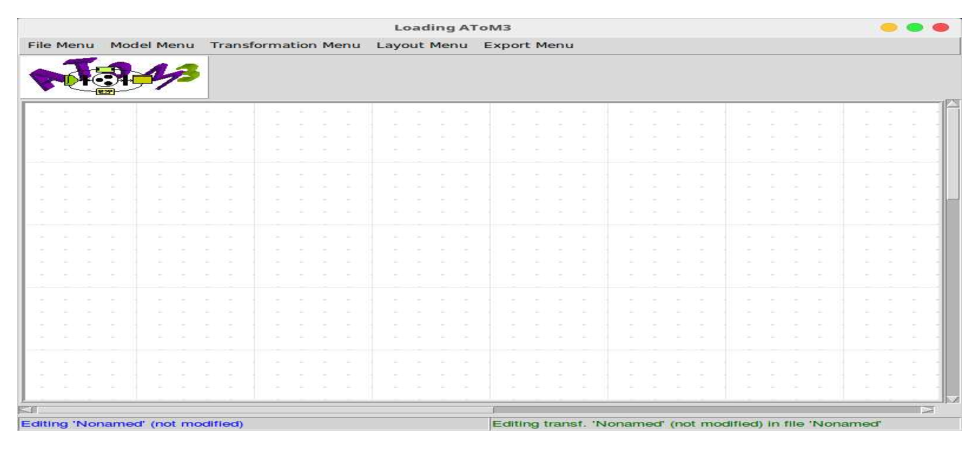
\includegraphics[scale=0.33]{ch3/img/atom3}
	\caption{\label{fig:AToM3 Window}AToM $^{3}$ Window}
\end{figure} 
\pagebreak
\subsection{Classes in AToM$^{3}$ }
In this work we use ClassDiagramm Formalism to create  our Formalism 
or Meta-Model is built in the tool so we can load it and use  it\cite{ch3-meta2}.
In AToM$^{3}$ the meta-models can be constructed from Classes and
Relationships.

The description of classes and association relations consists of

\begin{itemize}
\newcommand{\localtextbulletone}{\textcolor{gray}{\raisebox{.45ex}{\rule{.6ex}{.6ex}}}}
\renewcommand{\labelitemi}{\localtextbulletone}
\item  Name
\item  Attributes
\item  Constraints
\item  Action
\item  Cardinalities
\item  Appearance
\end{itemize}

\begin{figure}[th]
	\centering
		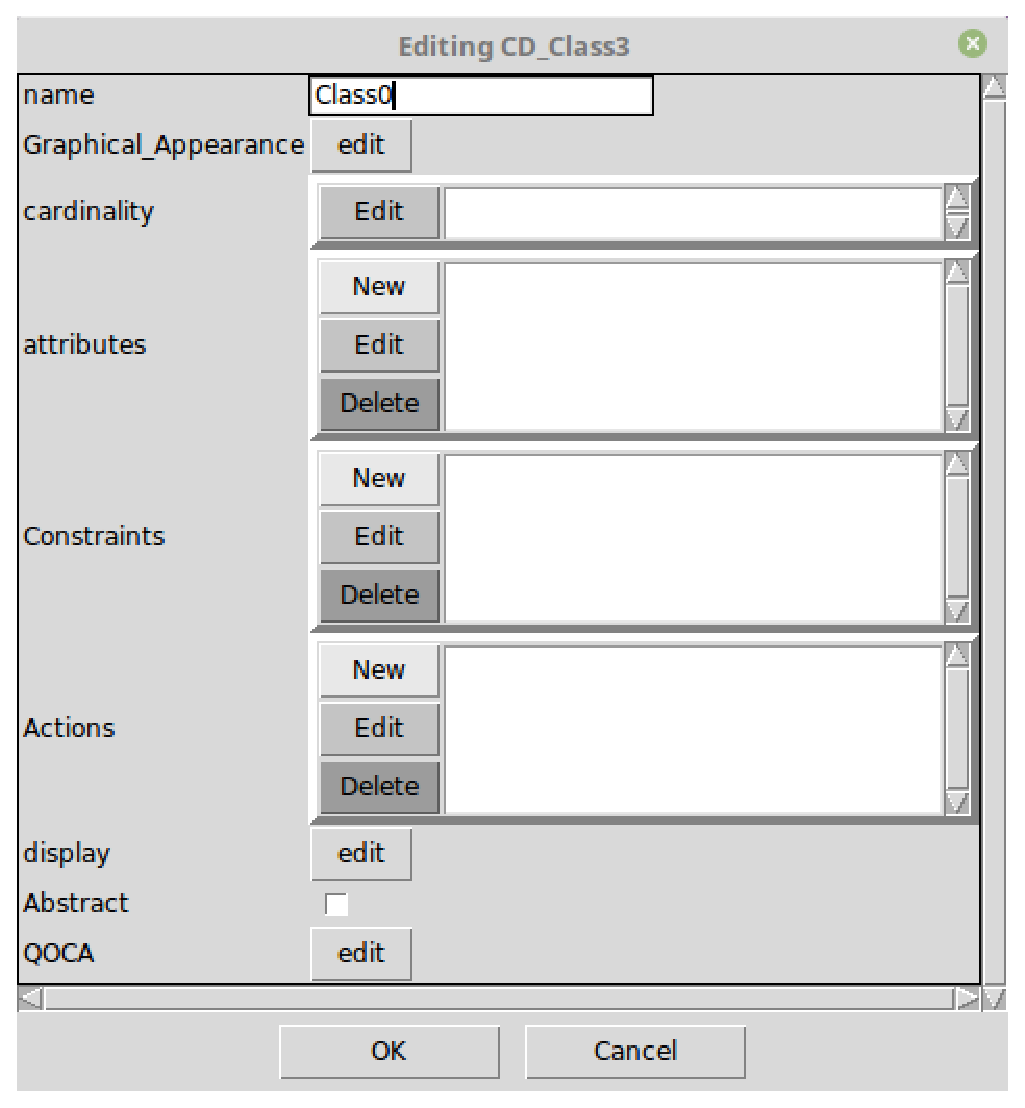
\includegraphics[scale=0.4]{ch3/img/class}
	\caption{\label{fig:Class Editor}Class Editor}
\end{figure} 

\subsubsection{ Constraint }

Constraints can be specified as OCL (Constraint Object Language) or Python
They have the following properties: 
\begin{itemize}
\newcommand{\localtextbulletone}{\textcolor{gray}{\raisebox{.45ex}{\rule{.6ex}{.6ex}}}}
\renewcommand{\labelitemi}{\localtextbulletone}
\item  constraint name
\item  triggering event  like Drag, Move, Select ..
and launch this event before (pre-condition) or after (post-condition)
 
\end{itemize}
 

\begin{figure}[th]
	\centering
	\includegraphics[scale=0.37]{ch3/img/const}
	\caption{\label{fig:Constraint Editor}Constraint Editor}
\end{figure} 
\subsubsection{ Action }

An action is similar to a constraint except that it has other effects and is a
Code in Pyton only, its have the same windows \ref{fig:Constraint Editor} 

They have the following properties :
\begin{itemize}
\newcommand{\localtextbulletone}{\textcolor{gray}{\raisebox{.45ex}{\rule{.6ex}{.6ex}}}}
\renewcommand{\labelitemi}{\localtextbulletone}
\item action name
\item triggering event: It can be either
	\begin{enumerate}
	\item Semantics such as saving a model
	\item Graphic or structural, such as moving or selecting an entity.
	\end{enumerate}
	
\item The execution is either
	\begin{enumerate}
	\item Before the event (precondition)
	\item  After (pots-condition) 
	\end{enumerate}

\end{itemize}
 


\subsection{Graph Grammer in AToM $^{3}$ }
In AToM3, grammar is a model characterized by
\begin{itemize}
\newcommand{\localtextbulletone}{\textcolor{gray}{\raisebox{.45ex}{\rule{.6ex}{.6ex}}}}
\renewcommand{\labelitemi}{\localtextbulletone}
\item An initial action.
\item A final action.
\item The set of rules. 
\end{itemize}
and this figure \ref{fig:Graph Grammar Window} Graph Grammar Editor
 
\begin{figure}[th]
	\centering 
	\includegraphics[scale=0.5]{ch3/img/GraphGrammar}
	\caption{\label{fig:Graph Grammar Window}Graph Grammar Window}
\end{figure} 
 

 Each rule consists of: 
\begin{itemize}
\newcommand{\localtextbulletone}{\textcolor{gray}{\raisebox{.45ex}{\rule{.6ex}{.6ex}}}}
\renewcommand{\labelitemi}{\localtextbulletone}
\item  A specific name for the rule.
\item  A priority indicating the order in which the rule is applied.
\item  A Left Hand Side (LHS) which is a graph.
\item  A right hand side (RHS) that can be a graph.
\item  A condition (Pyton code) that must be checked before the rule is
Applied.
\item An action (a Pyton code) that must be executed after the rule is
Applied
\end{itemize}


The rule editor figure \ref{fig:Rule Editor} allows the editing of the different parts of the rule as well as
The condition and action of each rule 
 
The condition editor and the action editor of a rule are similar to the editor of
Constraints presented in Figure \ref{fig:Constraint Editor}

\begin{figure}[th]
	\centering
 	\includegraphics[scale=0.38]{ch3/img/ruleEditor}
	\caption{\label{fig:Rule Editor}Rule Editor}
\end{figure} 
 

\section{PGraph Studio}   
PGraph Studio is a software that implements algorithms MSG, SSG, and ABB, and therefore, it is primarily
used as a solver for process synthesis problems. Furthermore, it is also capable of constructing process synthesis models.
As a modeling tool, it uses a tree-view that provides a clear overview of the actual problem under consideration and makes
it possible to edit the properties of multiple materials and operating units in parallel. The handling of measurement units
is aided with automated conversions. \cite{ ch3-pgraph2, Sitepgraph}


\begin{figure}[th]
	\centering  %[scale=1.2]
 	\includegraphics[scale=0.44]{ch3/img/pgraph}
	\caption{\label{fig:pgraphstudio)}P-Graph Studio Window }
\end{figure}  

As a solver, PNS Studio can generate the maximal structure, the combinatorial feasible structures, and the globally optimal
and suboptimal solutions of the problem. In the latter case the objective can be either cost minimization or profit max-
imization. PNS Studio provides a double pane view of solutions to compare alternatives.
Models and initial structures created in PNS Drawn can be imported into PNS Studio where they can be further edited. It
is also possible to export brief or more detailed reports from PNS Studio to Microsoft Excel \cite{ch3-pgraph}.
 

\chapter{\label{cha: Transformation Approach } Transformation Approach}
\section{Introduction}
Before start reading, i want to give you the main idea about this chapter. its contain our approach of transformation from omacs into pns in section \ref{sec:OMACS into PNS}, and the second approach in section \ref{sec:xml}, and the optimazation process in section \ref{sec:optim}.

\section{Implementation of the Transformation (OMACS into PNS)\label{sec:OMACS into PNS} }% Our Work
To Transform OMACS Model into PNS Model, we start to :
\begin{enumerate}
\item Define OMACS Meta-Model 
\item Define PNS Meta-Model
\item Define the rules of Transformation
\end{enumerate}


\subsection{OMACS} 
\subsubsection{Meta Model of OMACS}
\vspace{0.5cm}
To define OMACS meta model, we first load the Class Diagramm Formalism, to be able to create, manipulate our Meta-Model,
in OMACS Meta-Model contain set of classes:
\pagebreak
\begin{itemize}
	\item Agent  : we assign the work for this node (Entitie) to do 
	\item Capabilities : we add this node to the agent to be able to do a work
	\item Role : this is the work we assign for the agent 
	\item Goal : we want the agent reach this node 
\end{itemize}
 
\begin{figure}[th]
	\centering
 	\includegraphics[scale=0.7]{ch3/img/omacs_meta}
	\caption{\label{fig:OMACS Meta-Model}OMACS Meta-Model}
\end{figure} 
\vspace{0.9cm}
figure \ref{fig:OMACS Meta-Model} illustrate OMACS Meta-Model  contain 4 classes 
and 4 relation   
the Attribute Name in the classes represent the name of current node ,
and the rate attribute in the relation between classes represent  the relation percentage between two node or entities.

For example between an Agent and Capabilities its means how mush this Agent possese this capibilites
\pagebreak
\subsubsection{Example of OMACS}

Starting from  Meta-Model of OMACS in figure  \ref{fig:OMACS Meta-Model}, $AToM^3$ generate a formalism of OMACS, this formalism allow us to create our OMACS Model (Multi Agent System).
\vspace{0.1cm}
\begin{figure}[th]
	\centering
 	\includegraphics[scale=0.3]{ch3/img/omacs_model}
	\caption{\label{fig:OMACS Model}Formalism for OMACS Generated by $AToM^3$ }
\end{figure} 

Example in this figure \ref{fig:OMACS Model} represent a Multi Agent system which is  a component of 2 agent and 3 Capabilities, 2 Roles, 2 Goals

\subsection{PNS} 
\subsubsection{Meta Model of PNS}
To define PNS meta model, we first load the Class Diagramm Formalism, and its contain 4 classes and Relation
represent: 
\begin{itemize}
	\item Raw Material : represent a node does not have input arc 
	\item Intermediare Material 
	\item Final Product : this is the product of the system 
	\item Operating Unit : represent the task or operating which is consume the input material and produce the output material 
\end{itemize}
\pagebreak
\begin{figure}[th] 

	\centering
 	\includegraphics[scale=0.7]{ch3/img/pns_meta}
	\caption{\label{fig:PNS Meta-Model}PNS Meta-Model}
	
\end{figure} 

all material in figure \ref{fig:PNS Meta-Model} containt the same Attribute
\begin{itemize}


\item \textit{Name} : name of Material 
\item \textit{Price} : Price of Material
\item \textit{ReqFlow} : Requirment Flow means how much you have from this material in this system
\item \textit{MaxFlow} : Maximum Flow means how much your system can handle

\end{itemize}



and for the Operating Unit contain 3 Attribute : 
\begin{itemize}

\item Name : name of this Task 
\item Operating Cost Fix  : cost for entire period, Example : year
\item Operating Cost Proportional  :  cost for every Operating from this unit

\end{itemize}


\subsubsection{Example of PNS}
The  $AToM^3$ Tools  generate a formalism from the meta model we create before, load it and use it like figure \ref{fig:PNS Model} 

\begin{figure}[th]
	\centering
 	\includegraphics[scale=0.3]{ch3/img/pns_model}
	\caption{\label{fig:PNS Model}ToolBar for PNS Generated by $AToM^3$}
\end{figure} 

the previous figure \ref{fig:PNS Model} represent system de production contain 2 raw material and one intermediate material, final product and 3 operating unit.





\pagebreak
\subsection{Transformation Rules}
A Graph grammar is a grammar consisting of a set of rules, allow to 
Transform a formalisms of the same nature or of a different nature. 

Each Rule is composed of two parts, the left part (LHS) and the right part (RHS).
Each part can be a subgraph of the formalisms considered in the transformation

in our work, the formalisms considered in the transformation are formalism
OMACS as source graph to be transformed into PNS as target graph.

This grammar is defined using the AToM$^3$ tool according to the following step

\begin{enumerate}
	\item Load OMACS and PNS meta-models
	\item Create the transformation grammar
	\item Define the rules of grammar
	\item Generate the executable file of the grammar
\end{enumerate}

Our grammar is composed of :
\begin{description}
	\item [{Rules :}]  each rule is characterized
	by a name and execution priority. They are classified in 04 categories :
\end{description}


\paragraph{\emph{1)~Collect Categorie :} } 
Rules for Collect and create relation between some entitie
 
\paragraph{\emph{2)~Transform Categorie:} } 
Rules for transforming nodes or links into materials or operating units.
 

\paragraph{\emph{3)~Links Categorie:} } 
Rules to links generated materials and operating units 

\paragraph{\emph{4)~Cleaning Categorie:} } 
Rules to cleaning unnecessary entities from the result 

\end{enumerate}
our approach contain 20 rules, i mentions the most important transformation rules into the following steps  : 
\begin{itemize}

\item Create link between the agent and role depending on the common capabilites

\item Generate for every agent in OMACS Model into raw material in PNS Model
and the generated material has the same name and price 

\item Generate for every goal in OMACS Model into intermediate material in PNS Model and the generated material has the same name  


\item The product in the target graph which is PNS Model represent the organization of the OMACS Model

\item Create Operating unit for each direct link between the role and an agent 

\item Link the material was generated from goal with final product by operating unit

\end{itemize}


\paragraph{\emph{1)~Agent2RoleLink1 : Create the direct link  between the Agent and the Role (order 1) :} } The Figure \ref{fig:Create link between Agent and Role} illustrate how to create link between the agent and role depending on commun capabilities, order 1 mean it is the first rule applied in the grammar. 

\vspace{1cm}
\begin{figure}[th]
\centering
	\subfloat[LHS]{\includegraphics[scale=0.9]{ch3/img/L1}}
		\quad{}
		
\includegraphics{ch3/img/sep}
		\quad{}
	\subfloat[RHS]{\includegraphics[scale=0.9]{ch3/img/R1}}
\caption{\label{fig:Create link between Agent and Role}Assign Role to Agent } 
\end{figure}
 

\paragraph{\emph{2)~ TransAgent2Raw : Transform Agent to Raw Material (order 9) :} }
Application Of this rule in (figure \ref{fig:Generate for each agent raw material}) makes it possible to transform  every Agent in Multi Agent System into raw material, it has the same name and price.
\vspace{1cm}
\begin{figure}[th]
\centering
	\subfloat[LHS]{\includegraphics[scale=0.9]{ch3/img/L2}}
	\quad{}
		
\includegraphics{ch3/img/sep}
	\quad{}
	\subfloat[RHS]{\includegraphics[scale=0.9]{ch3/img/R2}}
\caption{\label{fig:Generate for each agent raw material}Transform Agent to Raw-material} 
\end{figure}
\vspace{1cm}

%% ------------------------------------------------------------------------------------------------ order 7 
\paragraph{\emph{3)~ TransLinkAR2OpUnit : Transform Link between Agent and Role into Operating Unit (order 10) :} } This rule (Figure \ref{fig:Operating Unit for every link capable of playing}) allow to transform, the relation capable of playing between an agent and role  into operating unit.
\vspace{1cm}
\begin{figure}[th]
	\centering
	\subfloat[LHS]{\includegraphics[scale=0.9]{ch3/img/L3}}
	\quad{}
		
\includegraphics{ch3/img/sep}
	\quad{}
	\subfloat[RHS]{\includegraphics[scale=0.9]{ch3/img/R3}}
\caption{\label{fig:Operating Unit for every link capable of playing}Transform CapableOf relation into operating unit} 
\end{figure}


%% ------------------------------------------------------------------------------------------------ order 9 
\paragraph{\emph{4)~ TransGoal2Mat : Transform Goal to intermediate material (order 11) :} }
Application of the rule illustrated in (Figure \ref{fig:Transform Goal to intermediate material}) Transform a goal in MaS into intermediate material in process system.
 
\begin{figure}[th]
\centering 
	\subfloat[LHS]{\includegraphics[scale=0.9]{ch3/img/L4}}
	\quad{}
		
\includegraphics{ch3/img/sep}
	\quad{}
	\subfloat[RHS]{\includegraphics[scale=0.9]{ch3/img/R4}}
\caption{\label{fig:Transform Goal to intermediate material}Transform Goal to intermediate material}
 
\end{figure}
\pagebreak
%% ------------------------------------------------------------------------------------------------ order 10 
\paragraph{\emph{5)~ CreateFinalStat : Create the Product node (order 13) :} }
Create the final material stat in the system like you notice the LHS is empty because this rule applied for one time, and this rule represented in 
(Figure \ref{fig:Create the final material} ).

\vspace{1cm}
\begin{figure}[th]
\centering
	\subfloat[LHS]{\includegraphics[scale=1.2]{ch3/img/empty_LHS}}% l5
	\quad{}
		
\includegraphics{ch3/img/sep}
	\quad{}
	\subfloat[RHS]{\includegraphics[scale=0.9]{ch3/img/R5}}
\caption{\label{fig:Create the final material}Create the final material}
 
\end{figure}
\vspace{1cm}

%% ------------------------------------------------------------------------------------------------ order  13
\paragraph{\emph{6)~ CreateMat_ARG : Generate auxiliary part  (order 14) :} }

The Application of this rule generate the auxiliary part which is intermediate material consumed by operating unit, and the auxiliary part represent an agent capable to playing role in order to achieve a specific goal, you can see that from (Figure \ref{fig:Generate auxiliary part}).
\vspace{1cm}
\begin{figure}[th]
\centering 
	\subfloat[LHS]{\includegraphics[scale=0.9]{ch3/img/L6}}
	\quad{}
		
\includegraphics{ch3/img/sep}
	\quad{}
	\subfloat[RHS]{\includegraphics[scale=0.9]{ch3/img/R6}}
\caption{\label{fig:Generate auxiliary part} Generate auxiliary part}
\end{figure}
\vspace{1cm}




%% ------------------------------------------------------------------------------------------------ order  15
\paragraph{\emph{7)~ CreateLinkMatr2OAF : Create Operating unit between goal material and the product (order 15) :} }
 
 
The rule in (Figure \ref{fig:Create Operating unit between  goal and OAF}) 
to Create an operating unit  between the final material and the goals material.
  
\vspace{1cm}
\begin{figure}[th]
\centering 
	\subfloat[LHS]{\includegraphics[scale=0.9]{ch3/img/L7}}
	\quad{}
		
\includegraphics{ch3/img/sep}
	\quad{}
	\subfloat[RHS]{\includegraphics[scale=0.9]{ch3/img/R7}}
\caption{\label{fig:Create Operating unit between  goal and OAF}Create Operating unit between  goal and OAF}
 
\end{figure}
\vspace{1cm}


%% ------------------------------------------------------------------------------------------------ order  19
\paragraph{\emph{8)~ CreateLinkMat_ARG2Goal : Create link between auxiliary part and  goal material  (order 19) :} }
 
 
The rule in (Figure \ref{fig:link between auxiliary part and goal})  describe 
how to link the auxiliary part with right goal.  


\begin{figure}[th]
\centering

	\subfloat[LHS]{\includegraphics[scale=2.2]{ch3/img/L8}}
	\quad{}\quad{}
		
\includegraphics{ch3/img/sep}
	\quad{}\quad{}
	\subfloat[LHS]{\includegraphics[scale=2.2]{ch3/img/R8}}
  
\caption{\label{fig:link between auxiliary part and goal}link between auxiliary part and goal}
 
\end{figure}
\pagebreak
%% ------------------------------------------------------------------------------------------------ order  20
\paragraph{\emph{9)~ CreatLinkRaw2AR : Create link to consume the raw material by operating unit  (order 20) :} }
 
 
This Figure \ref{fig:consume the raw material by operating unit}  illustrate  this rule, and it about how to create an arc between 
the raw material was generated from an agent and the operating unit.

\begin{figure}[th]
\centering
 	\subfloat[LHS]{\includegraphics[scale=2.9]{ch3/img/L9}}
		\quad{}\quad{}
			
\includegraphics{ch3/img/sep}
	\quad{}\quad{}
	\subfloat[LHS]{\includegraphics[scale=2.2]{ch3/img/R9}}
\caption{\label{fig:consume the raw material by operating unit} consume the raw material by operating unit}
\end{figure}

After that you notice some word in the rules like  :
\begin{itemize}
\item Left hand side
	\begin{enumerate}
	\item ANY : its attribue in the node and the engine will select every node with ANY attribute value
	\end{enumerate}
\item  Right hand side
	\begin{enumerate}
	\item COPIED : copie the attribue value from the node with same GGLabel in LHS
	\item SPECIFIED : specified the attribue value manualy or by code 
	\end{enumerate}
\end{itemize}
 
Now it's supposed to be aware every rule has a condition must be true  before the engine run this rule, i mention some these condition in the next part.
\pagebreak
\paragraph{\emph{1)~Condition for the rule   Assign Role to Agent  :  } } 
 
Test if there is a node agent, role visited before 
in order not to fall in infinity loop, figure \ref{fig:Create link between Agent and Role} represent the rule.
 
\begin{figure}[th]
	\centering
 	\includegraphics[scale=0.37]{ch3/img/condrule1}
	\caption{\label{fig:Condition link agent with role}Condition link agent with role  }
\end{figure} 

\paragraph{\emph{2)~Condition for Create Final Stat : } } 
This conditon test if this attribute Final stat equal zero 
, in other word we did not visite this rule before, the rule in figure\ref{fig:Create the final material}.
 
 
\vspace{1cm}
\begin{figure}[th]
	\centering
 	\includegraphics[scale=0.37]{ch3/img/condfinal}
	\caption{\label{fig:Condition of generate final stat } Condition of generate final stat }
\end{figure} 
 

\paragraph{\emph{3)~Condition of rule link between AUX part and Material Goal } : }
Here we check if we did not visited before  and the name of Auxiliary Part end with goal name to link it with the right goal material, the rule in figure \ref{fig:link between auxiliary part and goal}.
 
\vspace{1cm}
 
\begin{figure}[th]
	\centering
 	\includegraphics[scale=0.37]{ch3/img/condaux}
	\caption{\label{fig:Condition of Auxiliary part}Condition of Auxiliary part  }
\end{figure} 
\pagebreak

\subsection{Examples }

\subsubsection{Simple multi Agent System }
This example represents a very simple system composed of  two agent and 3 capabilities, 2 role and 2 goals.
 Figure \ref{fig:Example 1 Multi Agent System } illustrates this example :
\begin{figure}[th]
	\centering
 	\includegraphics[scale=0.3]{ch3/img/omacs_model}
	\caption{\label{fig:Example 1 Multi Agent System }Example 1 Multi Agent System}
\end{figure} 
\pagebreak
The purpose of this example is to demonstrate the transformation of multi agent system in OMACS into pns model

Figure \ref{fig:Multi Agent System After transformation } shows the transformation result.
It is clear that the resulting contain set of material and operating unit
 
\begin{itemize}
\item The raw material A1, A2 represent the agent  
\item The operating unit A1 R1 represent the relation between an A1 and R1 
in Mas before the transformation its the same for other entities like this one
\item the operating unit and material named A2 R2 G2 represent agent A2 Playing R2 in order to achieve G2, it is the same for other entities  

\item the operating unit and material named A2 R2 G2 represent agent A2 Playing R2 in order to achieve G2 


\item the operating unit and material named A1 R1 G2 represent agent A1 Playing R1 in order to achieve G2  and G2, any agent in this is capable to play R1 can reach G1 and G2
 

\end{itemize}
  


\begin{figure}[th]
	\centering
 	\includegraphics[scale=0.3]{ch3/img/ex1pns}
	\caption{\label{fig:Multi Agent System After transformation }Multi Agent System After transformation}
\end{figure}  
\pagebreak
\subsubsection{ Complex multi Agent System }
This example represents a complex system composed of  3 agent and 4 capabilities, 2 role and 4 goals. Figure \ref{fig:Example 1 Multi Agent System } illustrates this example ,
 


\begin{figure}[th]
	\centering
 	\includegraphics[scale=0.3]{ch3/img/article}
	\caption{\label{fig:Complex Multi Agent System}Complex Multi Agent System}
\end{figure} 

\begin{itemize}
	\item every agent possesses set of capabilites for example A1 possese all capabilies in the system
	\item Role require list of capabilies every agent has the same capabilies or more, so he can play this role
	\item Role R1, R2 achieve all goal in the system
	\item the Agent A1 all capabilites in the system so we can say, A1 capable of playing R1 and R2
	\item Agent A1 capable of playing all roles in this system, so he can achieve all goal in the system
\end{itemize}
\vspace{2cm}

after the Transformation of Multi agent system from OMACS frame into PNS framework we get this model in figure \ref{fig:Complex Multi Agent System After transforamtion} 
and next table represent the value of this model 

 % Please add the following required packages to your document preamble:
% \usepackage{booktabs}

\begin{table}[h!]
\centering
\begin{tabular}{@{}ccc@{}}
\toprule
\textbf{Operating Unit} & \textbf{Input Material} & \textbf{Output Material}                                                                              \\ \midrule
G1OAF                   & G1(1)                   & OAF (1)                                                                                               \\
G2OAF                   & G2(1)                   & OAF(1)                                                                                                \\
G3OAF                   & G3(1)                   & OAF(1)                                                                                                \\
G4OAF                   & G4(1)                   & OAF(1)                                                                                                \\ \midrule
A1R1G1                  & A1R1G1(0.433)           & G1(0.2)                                                                                               \\
A1R1G2                  & A1R1G2(0.433)           & G2(0.4)                                                                                               \\
A1R1G3                  & A1R1G3(0.433)           & G3(0.6)                                                                                               \\
A1R1G4                  & A1R1G4(0.433)           & G4(0.8)                                                                                               \\
A1R2G1                  & A1R2G1(0.433)           & G1(1.0)                                                                                               \\
A1R2G2                  & A1R2G2(0.433)           & G2(0.7)                                                                                               \\
A1R2G3                  & A1R2G3(0.433)           & G3(0.4)                                                                                               \\
A1R2G4                  & A1R2G4(0.433)           & G4(0.1)                                                                                               \\
A2R2G1                  & A2R2G1(0.633)           & G1(1.0)                                                                                               \\
A2R2G2                  & A2R2G2(0.633)           & G2(0.7)                                                                                               \\
A2R2G3                  & A2R2G3(0.633)           & G3(0.4)                                                                                               \\
A2R2G4                  & A2R2G4(0.633)           & G4(0.1)                                                                                               \\
A3R2G1                  & A3R2G1(0.5)             & G1(1.0)                                                                                               \\
A3R2G2                  & A3R2G2(0.5)             & G2(0.7)                                                                                               \\
A3R2G3                  & A3R2G3(0.5)             & G3(0.4)                                                                                               \\
A3R2G4                  & A3R2G4(0.5)             & G4(0.1)                                                                                               \\ \midrule
A1R1                    & A1                      & \begin{tabular}[c]{@{}c@{}}A1R1G1(0.433) ,A1R1G2(0.433) \\ ,A1R1G3(0.433) ,A1R1G4(0.433)\end{tabular} \\ \midrule
A1R2                    & A1                      & \begin{tabular}[c]{@{}c@{}}A1R2G1(0.433) ,A1R2G2(0.433) ,\\ A1R2G3(0.433) ,A1R2G4(0.433)\end{tabular} \\ \midrule
A2R2                    & A2                      & \begin{tabular}[c]{@{}c@{}}A2R2G1(0.633) ,A2R2G2(0.633) ,\\ A2R2G3(0.633) ,A2R2G4(0.633)\end{tabular} \\ \midrule
A3R2                    & A3                      & \begin{tabular}[c]{@{}c@{}}A3R2G1(0.5) ,A3R2G2(0.5) ,\\ A3R2G3(0.5) ,A3R2G4(0.5)\end{tabular}         \\ \bottomrule
\end{tabular}

\caption{Value of PNS Model}
\label{Value of PNS Model}
\end{table}


% Add table HEre
 \begin{landscape}
\begin{figure}[th]
	\centering 
 	\includegraphics[scale=1.3]{ch3/img/articlePNS2}
	\caption{\label{fig:Complex Multi Agent System After transforamtion}Complex Multi Agent System After transforamtion}
\end{figure} 
 
 \end{landscape}


% now we have the MaS in PNS Form 
% and there Tools called PGraphStudio
%
%
\section{Transformation Approach ( PNS into XML file )\label{sec:xml} }
In Section \ref{sec:OMACS into PNS} we presented our transformation approach That allows 
to transform the OMACS to PNS.

The purpose of this transformation is the Optimization and for this we
Proposed Another processing approach That transforms PNS to XML 
files to analysis for a optimization tool 
\subsection{ Graph Grammar }
 this grammar is Composed of three parts: 
\begin{itemize}
\item \textbf{Initial Action : } This portion of our grammar is used to initialize all
Global variables used. They are used to meet various needs.  in Figure \ref{fig:Code Initial Action} 

\end{itemize}

\begin{figure}[th]
	\centering  %[scale=1.2]
 	\includegraphics[scale=0.38]{ch3/img/InitAct}
	\caption{\label{fig:Code Initial Action}Code Initial Action}
\end{figure} 

\begin{itemize}
\item \textbf{Final Action : } Final Action Allows Completing the.xml file by the tags
XML Completing the after-processing of all PNS nodes and save the page name. in figure \ref{fig:Code Final Action} 
   
\end{itemize}

\begin{figure}[th]
	\centering  %[scale=1.2]
 	\includegraphics[scale=0.38]{ch3/img/FinAct}
	\caption{\label{fig:Code Final Action}Code Final Action}
\end{figure} 
\pagebreak
\begin{itemize}
\item \textbf{ Set of Rules : } 
 
Our grammar graphs Consists of ten rules. Each
rule is Characterized by a name and an execution priority. 

\end{itemize}
 We quote here The Most major rules: 
\paragraph{\emph{1)~Transform RawMaterial into XML code :} }
This rule (Figure \ref{fig:Raw Material into Xml}) to priority equal to "1", ie, 
it is the first rule applied on the Model. She transforms the place into a XML

\begin{figure}[th]
\centering

\subfloat[LHS]{\includegraphics[scale=0.5]{ch3/img/xL1}}
\quad{}
\includegraphics{ch3/img/sep}
\quad{}
\subfloat[RHS]{\includegraphics[scale=0.5]{ch3/img/xR1}}
 
 
\caption{\label{fig:Raw Material into Xml}Raw Material into Xml} 

\end{figure} 

\paragraph{\emph{ a )~Condition for rule \ref{fig:Raw Material into Xml} } } For the application of this rule, it must be verified that the partition To be transformed is not treated before

\begin{figure}[th]
	\centering  %[scale=1.2]
 	\includegraphics[scale=0.38]{ch3/img/xcond1}
	\caption{\label{fig:condition of Raw Material for Transfromation}condition of Raw Material for Transfromation}
\end{figure}
\paragraph{\emph{ b )~Action for rule \ref{fig:Raw Material into Xml} } }  Once the rule is applied, it Action Allows to create a code INSTEAD XML and mark the object to the left side to processed.  
 
\begin{figure}[th]
	\centering  %[scale=1.2]
 	\includegraphics[scale=0.38]{ch3/img/xact1}
	\caption{\label{fig:Action of Raw Material for Transfromation}Action of Raw Material for Transfromation}
\end{figure} 
\vspace{1cm}
like you see in the first line i import MyFunction is external file, Python code 
to be easy to manipulate  and this is the function to add new material ( raw, intermadiate, final)
and for the operating unit is the similair function
 
\vspace{1cm}
\begin{lstlisting}[language=Python, caption=Python Function Material]
def newMaterial(  parent=None, name= "None", ID="0", Type= "None", xN ='-1', yN ='-1' ,price='-1' ,reqF = 0  ,maxF =999999 ):
	#Create new Node has the Material Name...and add it into the parent node
	node = ET.SubElement(parent, "Material",ID=str(ID),Name=name,Type=str(Type))
    print 'add Cords into node		-NewNode-'
	#Create Corde for the node material
	cords = ET.SubElement(node, "Coords")
	ET.SubElement(cords, "X").text = str( xN )
	ET.SubElement(cords, "Y").text = str( yN )
	#Test if the patameter is not null or empty
	if price != '-1' or  reqF != 0  or maxF !=999999 : 
		ParameterList = ET.SubElement(node, "ParameterList")
		ET.SubElement(ParameterList, "Parameter",Name="price",Value=str( price) )
		if reqF == 0 : reqF = '-1'
		ET.SubElement(ParameterList, "Parameter",Name="reqflow",Value= str(reqF) )
		if maxF == 999999 : maxF = '-1'
		ET.SubElement(ParameterList, "Parameter",Name="maxflow",Value=str(maxF) )

	#Create Label for the MaterialNode
	label = ET.SubElement(node, "Label",Text = str(name))
	offset = ET.SubElement(label,  "Offset")
	ET.SubElement(offset, "X").text =   str(5)
	ET.SubElement(offset, "Y").text =   str(0)
	
	return node
\end{lstlisting}

\paragraph{\emph{2)~Transform Edge between two entitie into XML code :} } in this transformation 
we want to create link between nodes Material and Operating unit 
and we have  4 type of Edges : 
\begin{itemize}
	\item Edges from raw material into Operating unit
	\item Edges from intermediate material into Operating unit
	
	\item Edges from  Operating unit into final material
	\item Edges from  Operating unit into intermadiate material 
\end{itemize}
and the figure \ref{fig:edgotoraw} represent the first Edge type 

\begin{figure}[th]
\centering
 \subfloat[LHS]{\includegraphics[scale=1.3]{ch3/img/xL2}}
 \quad{} \quad{}
\includegraphics{ch3/img/sep}
\quad{} \quad{}
\subfloat[RHS]{\includegraphics[scale=1.3]{ch3/img/xR2}}

\caption{\label{fig:edgotoraw}Edges from Raw Material into Operating unit to xml code} 

\end{figure} 
  
\paragraph{\emph{ a )~Condition for rule \ref{fig:edgotoraw} } } it is the same with figure \ref{fig:condition of Raw Material for Transfromation} but here we select the edges

\vspace{1cm} 
\begin{figure}[th]
	\centering  %[scale=1.2]
 	\includegraphics[scale=0.38]{ch3/img/xcond2}
	\caption{\label{fig:Condition2)}Condition of Edges ( RawMaterial to Operating unit)}
 \end{figure} 
\vspace{1cm}
\paragraph{\emph{ b )~Action for rule \ref{fig:edgotoraw} } }  we add this action to  Transform the Edges between Any Material and Any Operating unit into xml file, or to export the entitie from Graphical presentation 
into Xml Code  
\pagebreak 


\begin{figure}[th]
	\centering  %[scale=1.2]
 	\includegraphics[scale=0.38]{ch3/img/xact2}
	\caption{\label{fig:action2)}Action of Edges ( RawMaterial to Operating unit)}
\end{figure}  

and this code represent a Function to add new Edges into the Tree code 
to export the tree later 

\begin{lstlisting}[language=Python, caption=Python Function new Edges]
def newEdges(  parent, name, ID, xN, yN    ,beginID, endID    ):
	#Create new Node and add it into parent Node	
	node = ET.SubElement(parent, "Edge",ID=str(ID),BeginID=str(beginID),EndID=str(endID),Rate=str(name),Title=str(name), ArrowOnCenter="true", ArrowPosition="50")  
	
	#Create Corde for the node Edges
	cords = ET.SubElement(node, "Coords")
	ET.SubElement(cords, "X").text = str( xN )
	ET.SubElement(cords, "Y").text = str( yN )
		 		 		  
	#Create Label for the Edges
	label = ET.SubElement(node, "Label",Text = str(name))
	offset = ET.SubElement(label,  "Offset")
	ET.SubElement(offset, "X").text =   str(5)
	ET.SubElement(offset, "Y").text =   str(0)
 
	return node 
\end{lstlisting}

% UPDATE 13.47

\pagebreak
\section{Optimisation Multi Agent System \label{sec:optim} }

To optimize the multi-agent system in  Process Process synthesis, we chose tool called  P-Graph Studio 

\textbf{P-Graph Studio : }   is a software that implements algorithms MSG, SSG, and ABB, and therefore, it is primarily
used as a solver for process synthesis problems. Furthermore, it is also capable of constructing process synthesis models.
As a modeling tool, it uses a tree-view that provides a clear overview of the actual problem under consideration and makes
it possible to edit the properties of multiple materials and operating units in parallel. The handling of measurement units
is aided with automated conversions. \cite{ ch3-pgraph2, Sitepgraph}

As a solver, PNS Studio can generate the maximal structure, the combinatorial feasible structures, and the globally optimal
and suboptimal solutions of the problem. In the latter case the objective can be either cost minimization or profit max-
imization. PNS Studio provides a double pane view of solutions to compare alternatives.
Models and initial structures created in PNS Drawn can be imported into PNS Studio where they can be further edited. It
is also possible to export brief or more detailed reports from PNS Studio to Microsoft Excel. \cite{ch3-pgraph}

\begin{figure}[th]
	\centering  %[scale=1.2]
 	\includegraphics[scale=0.44]{ch3/img/pgraph}
	\caption{\label{fig:pgraphstudio)}P-Graph Studio Window }
\end{figure}  


figure \ref{fig:Multi Agent System in PGraph Studio} represent multi agent system, Previously mentioned in figure \ref{fig:Complex Multi Agent System After transforamtion} 
\begin{figure}[th]
	\centering
		\includegraphics[scale=0.44]{ch3/img/pgraphArt}
	\caption{\label{fig:Multi Agent System in PGraph Studio}Multi Agent System in PGraph Studio}
\end{figure} 
\pagebreak
After we use this tool to optimise, we got this figure \ref{fig:Multi Agent System in Optimum structure}

\begin{figure}[th]
	\centering
		\includegraphics[scale=0.44]{ch3/img/pgraphSol}
	\caption{\label{fig:Multi Agent System in Optimum structure}Multi Agent System in Optimum structure}
\end{figure} 

PGraph Studio Generate 2 Files : 
\begin{itemize}
	\item Graph.in and contain :
		\begin{enumerate}
			\item information about Material, price, quanity
			\item information about operating unit, income material and outcome material 
 	\end{enumerate}

\end{itemize}

\begin{lstlisting}[caption=Part from Graph.in]
material_to_operating_unit_flow_rates:

A1_R1: A1 => 0.433 A1_R1_G1 + 0.433 A1_R1_G4 +
			 0.433 A1_R1_G3 + 0.433 A1_R1_G2
A1_R2: A1 => 0.433 A1_R2_G4 + 0.433 A1_R2_G3 + 
			 0.433 A1_R2_G2 + 0.433 A1_R2_G1
A2_R2: A2 => 0.633 A2_R2_G4 + 0.633 A2_R2_G3 + 
			 0.633 A2_R2_G2 + 0.633 A2_R2_G1
A3_R2: A3 => 0.5 A3_R2_G4 + 0.5 A3_R2_G3 + 
			 0.5 A3_R2_G2 + 0.5 A3_R2_G1
			 
G1_OAF: G1 => OAF
G2_OAF: G2 => OAF
G3_OAF: G3 => OAF
G4_OAF: G4 => OAF

\end{lstlisting}



\begin{itemize}
	\item Graph.out and contain :
		\begin{enumerate}
			\item All possible solution, starting with the optimum solution 
			\item every solution presented by set of  operating unit, material and consumtion rate  
 	\end{enumerate}

\end{itemize}



\begin{lstlisting}[caption=Part from Graph.out]
Feasible structure #2:
Materials:

A2 (64.6273 EUR/y): -0.718081 g/y
A2_R2_G1: balanced
A2_R2_G2: balanced
A2_R2_G3: balanced
A2_R2_G4: balanced
G1: balanced
G2: balanced
G3: balanced
G4: balanced
OAF (-0 EUR/y): 1 g/y

Operating units:

0.718081*A2_R2 (0.454545 EUR/y): 
		A2 (-0.718081 g/y) =>  A2_R2_G1 (0.454545 g/y) A2_R2_G2 (0.454545 g/y) 
								A2_R2_G3 (0.454545 g/y) A2_R2_G4 (0.454545 g/y) 
								
0.454545*G1_OAF (2.45455 EUR/y): G1 (-0.454545 g/y) => OAF (0.454545 g/y) 
0.318182*G2_OAF (2.31818 EUR/y): G2 (-0.318182 g/y) => OAF (0.318182 g/y) 
0.181818*G3_OAF (2.18182 EUR/y): G3 (-0.181818 g/y) => OAF (0.181818 g/y) 
0.045454*G4_OAF (2.04545 EUR/y): G4 (-0.045454 g/y) => OAF (0.045454 g/y) 

0.454545*A2_R2_G3 (2.18182 EUR/y): 
				A2_R2_G3 (-0.454545 g/y) =>   G3 (0.181818 g/y) 
				
0.454545*A2_R2_G2 (2.31818 EUR/y):
				A2_R2_G2 (-0.454545 g/y) =>   G2 (0.318182 g/y) 
				
0.454545*A2_R2_G1 (2.45455 EUR/y): 
				A2_R2_G1 (-0.454545 g/y) =>  G1 (0.454545 g/y) 
				
0.454545*A2_R2_G4 (2.04545 EUR/y): 
				A2_R2_G4(-0.454545 g/y) => G4 (0.0454545 g/y) 
Total annual cost= 83.0819 EUR/y


\end{lstlisting}

\section{Conclusion}
We have presented in this chapter the principles of graph transformations and then we have presented our approach of transformations of the multi agent system in OMACS frame work to PNS, And we also presented our 2nd
approach that transforms PNS Model  into XML file after that we saw the tool
PGraph Studio we use it to optimize multi agent system in pns frame work.

% 23:47 khmiss


\chapter*{General Conclusion}

\addcontentsline{toc}{chapter}{\numberline{}{General Conclusion}}

Through our project, We explained the aim of our project wchich is to find the optimum organization of multi agent system, and this later represented according the OMACS framework.

We have introduced in the first chapter, Motivation and some concept of organization and reorganization in MaS and we presented two frameworks (OMACS, PNS), that allow us to design a MaS.

The Second chapter was about the PGraph Framework and Process Network Synthesis, the basic concept and mathematical definition  of this framework, and we mentioned 
three algorithm applicable on PNS 

In the Third chapter, we explained the concept of model transformation approaches and we concentrated on the Graph transformation approach, followed by an overview about the Tool AToM3, it allow us to define the meta model and generate a formalism from these meta model.

In the fourth chapter, we presented our approach to transform a MaS modeled in OMACS presentation into PNS Model, and 
we defined the meta model for both frameworks (OMACS, PNS), 
we propose two approach, the (OMACS TO PNS) approach, to transform OMACS model into PNS model, and the second approach  to transform the generated ons model by the first approach into XML file, to be able to apply ABB in PGraph Studio to find the best (optimum) structure.

Our work depend on a tool called PGraph studio, to apply the (Branch \& Bound) algorithm, because of that we propose as a perspective to implement ABB algorithm using graph grammar to make our approaches autonomous.

\backmatter
\pagestyle{plain}

\phantomsection
\addcontentsline{toc}{chapter}{\numberline{}{Bibliographie}}
%\addcontentsline{toc}{section}{References}
 
\bibliographystyle{ieeetr}
\bibliography{b}
 
 

 
\setcounter{figure}{0}
 
\end{document}

% 0200 kmiss
